\documentclass{article}

\usepackage{amsmath}
\usepackage{palatino}
\usepackage{tikz}

\newcommand{\diag}{\Delta}
\newcommand{\ccat}{\mathbf{C}}
\newcommand{\id}{\emph{id}}
\newcommand{\pow}{\mathcal{P}}
\newcommand{\fpow}{\mathbf{\mathcal{P}}}
\newcommand{\cset}{\mathbf{Set}}
\newcommand{\eval}{\emph{eval}}
\newcommand{\curry}{\emph{curry}}
\newcommand{\natarrow}{\dot{\rightarrow}}
\newcommand{\fhom}{\mathbf{hom}}

\newcommand{\pcat}{\mathbf{P}}

\begin{document}

\begin{enumerate}
\item [2.3.11.1]
  The diagram from Pierce's example 2.3.4 argued that $\eval : F_A \natarrow I_\cset$ was a natural transformation.
  Proof follows if the following diagram commutes for a fixed set $A$ and every arrow $g : C \rightarrow B$.
  \begin{center}
    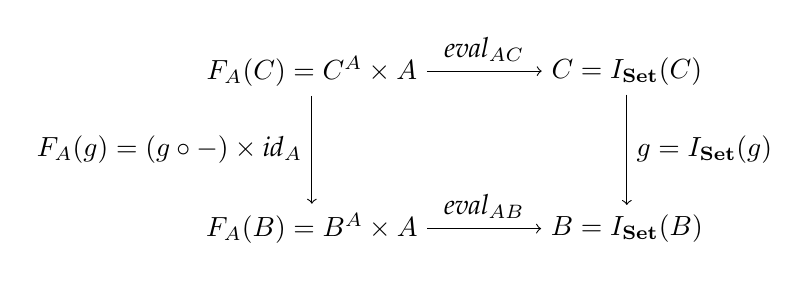
\begin{tikzpicture}
      \node (1) {$F_A(C) = C^A \times A$};
      \node[right of=1,xshift=3cm] (2) {$C = I_\cset(C)$};
      \node[below of=1,yshift=-1cm] (3) {$F_A(B) = B^A \times A$};
      \node[below of=2,yshift=-1cm] (4) {$B = I_\cset(B)$};

      \draw[->] (1) -- node[above] {$\eval_{AC}$} (2);
      \draw[->] (2) -- node[right] {$g = I_\cset(g)$} (4);
      \draw[->] (1) -- node[left] {$F_A(g) = (g \circ -) \times \id_A$} (3);
      \draw[->] (3) -- node[above] {$\eval_{AB}$} (4);
    \end{tikzpicture}
  \end{center}
  We need to show that $g \circ \eval_{AC} = \eval_{AB} \circ (g\circ -) \times \id_A$, and we can prove this by using the universal property of $\eval_{AB}$.
  
\subitem
  The exponential object $B^A$ and arrow $\eval_{AB}$ guarantee that for every arrow $h : C^A \times A \rightarrow B$, we can derive an arrow $C^A \times A \rightarrow B^A \times A$ by currying $h$.
  Take $h = g \circ \eval_{AC} : C^A \times A \rightarrow B$.
  We see that the following diagram commutes.
  \begin{center}
    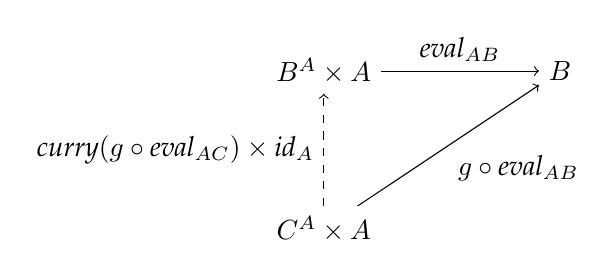
\begin{tikzpicture}
      \node (1) {$B^A \times A$};
      \node[right of=1,xshift=2cm] (2) {$B$};
      \node[below of=1,yshift=-1cm] (3) {$C^A \times A$};
      
      \draw[->] (1) -- node[above] {$\eval_{AB}$} (2);
      \draw[->] (3) -- node[below right] {$g \circ \eval_{AB}$} (2);
      \draw[->,dashed] (3) -- node[left] {$\curry(g \circ \eval_{AC}) \times \id_A$} (1);
    \end{tikzpicture}
  \end{center}
  Filling in the blank above in the arrow $F_A(g) = (g \circ -) \times \id_A$, we see that $(g \circ -) = (g \circ \eval_{AC})$.
  Therefore the diagram from example 2.3.4 commutes, proving that $\eval : F_A \natarrow I_\cset$ is a natural transformation.
\newpage

\item [2.3.11.2]
  Let $\pcat$ be a preorder regarded as a category, let $\ccat$ be an arbitrary category, and let $S,T : \ccat \rightarrow \pcat$ be functors.
  We show that there is a unique natural transformation $\tau : S \natarrow T$ if and only if for all $\ccat$ objects $C$, the relationship $S(C) \le T(C)$ holds.

\subitem
  First assume that $\tau$ is a unique natural transformation.
  This implies that for any $\ccat$ arrow $f : A \rightarrow B$, there exist arrows $\tau_A: S(A) \rightarrow T(A)$ and $\tau_B : S(B) \rightarrow T(B)$.
  Let $f$ stand for an arbitrary identity arrow $\id_C : C \rightarrow C$ in $\ccat$.
  We see that there exists $\tau_C : S(C) \rightarrow T(C)$.
  This is an arrow in $\pcat$, thus the inequality $S(C) \le T(C)$ holds for arbitrary objects $C$ in $\ccat$.

\subitem
  Next assume that for every $\ccat$-object $C$, we have that $S(C) \le T(C)$.
  This inequality implies that there exists a $\pcat$-arrow $f : S(C) \rightarrow T(C)$.
  Now consider a $\ccat$-arrow $f : A \rightarrow B$.
  We know that there exist arrows $S(A) \rightarrow T(A)$ and $S(B) \rightarrow T(B)$ in $\pcat$.
  %% TODO questionable
  Furthermore, these arrows are uniquely determined by $f$.
  Hence $\tau$ in the following diagram is a unique natural transformation between $S$ and $T$.
  \begin{center}
    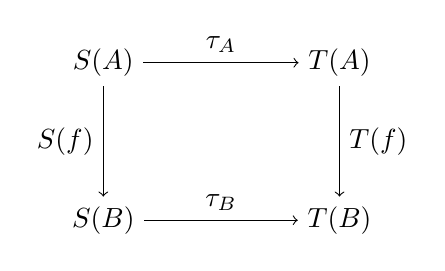
\begin{tikzpicture}
      \node (1) {$S(A)$};
      \node[right of=1,xshift=2cm] (2) {$T(A)$};
      \node[below of=1,yshift=-1cm] (3) {$S(B)$};
      \node[below of=2,yshift=-1cm] (4) {$T(B)$};

      \draw[->] (1) -- node[above] {$\tau_A$} (2);
      \draw[->] (1) -- node[left] {$S(f)$} (3);
      \draw[->] (2) -- node[right] {$T(f)$} (4);
      \draw[->] (3) -- node[above] {$\tau_B$} (4);
    \end{tikzpicture}
  \end{center}

\item[]
\item [2.3.11.3]
  The identity functor $I_\cset : \cset \rightarrow \cset$ is represented by any singleton set because a singleton set is an initial object in the category $\cset$.
  Let $R$ stand for an arbitrary singleton set and consider the functors $I_\cset$ and $\fhom(R,-)$, the identity functor on $\cset$ and the hom-functor defined by the singleton $R$.
  These functors define the following arrows for each $\cset$-arrow $f : A \rightarrow B$.
  \begin{center}
    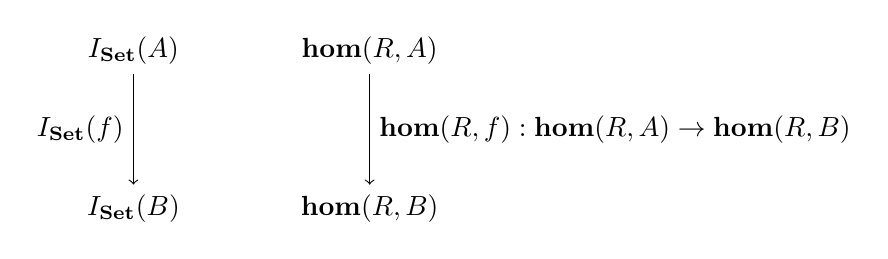
\begin{tikzpicture}
      \node (1) {$I_\cset(A)$};
      \node[right of=1,xshift=2cm] (2) {$\fhom(R,A)$};
      \node[below of=1,yshift=-1cm] (3) {$I_\cset(B)$};
      \node[below of=2,yshift=-1cm] (4) {$\fhom(R,B)$};

      \draw[->] (1) -- node[left] {$I_\cset(f)$} (3);
      \draw[->] (2) -- node[right] {$\fhom(R,f) : \fhom(R,A) \rightarrow \fhom(R,B)$} (4);
    \end{tikzpicture}
  \end{center}
  
  Because $R$ is a singleton, there exists one unique arrow in each hom-set $\hom(R,A)$.
  Furthermore, there is one hom-set for each $\cset$-object $A$, therefore we have an isomorphism between $\cset$ objects and the unique arrows to these objects from the singleton $R$.
  This natural isomorphism proves that $I_\cset$ is represented by the singleton set $R$.

\newpage
\item [2.3.11.4]
\item [2.3.11.5]
\end{enumerate}
\end{document}
